\section{Entwicklung der Anwendung}\label{sec:entwicklung}

In Kapitel~\ref{sec:grundlagen} und~\ref{sec:architektur} wurden die notwendigen Grundlagen und die Architektur vermittelt.
Darauf aufbauend wird in den folgenden Abschnitten ein tieferer Einblick in die Entwicklungsphase vorgenommen und dazu passend Teile des Codes vorgestellt.
Dazu ist dieses Kapitel in vier Abschnitte gegliedert, in denen jeweils eine Komponente der Anwendung behandelt wird.

\subsection{Erste Komponente: E-Graph}

Die Erstellung eines E-Graphs beginnt mit einem mathematischen Ausdruck, aus dem ein \textbf{Abstract Syntax Tree} (AST) aufgebaut wird.
Der AST wird später traversiert, um jeden Knoten dem E-Graph hinzuzufügen. Dieser Zwischenschritt vereinfacht die Erzeugung von E-Graphs und
kann gleichzeitig als Validierungsphase genutzt werden, da hier bereits feststeht, ob der Ausdruck der korrekten Form entspricht.

\subsubsection{AbstractSyntaxTree \& AbstractSyntaxTreeNode}

Ein AST erfordert die Klassen \textit{AbstractSyntaxTreeNode} (Listing~\ref{lst:astnode}) und 
\textit{AbstractSyntaxTree} (Listing~\ref{lst:ast}). Die Klasse \textit{AbstractSyntaxTreeNode} repräsentiert
einen Knoten im AST. Sie hat drei Attribute: einen linken Zeiger, einen rechten Zeiger und einen Schlüssel.

\begin{lstlisting}[language=Python, caption=Klasse \textit{AbstractSyntaxTreeNode}, label={lst:astnode}]
class AbstractSyntaxTreeNode:
    def __init__(self):
        self.left = None
        self.key = str()
        self.right = None
\end{lstlisting}

Der Schlüssel kann eine arithmetische Operation, eine Variable oder eine Zahl sein. Die Zeiger können auf einen weiteren Teilbaum zeigen, auf einen einzelnen Knoten
oder auf nichts. Mithilfe dieser Klasse kann nachher ein ganzer Baum dargestellt werden. Dazu braucht man nur den Wurzelknoten des Baumes abspeichern, um über dessen Kinder
Zugriff auf den gesamten Baum zu bekommen. 

Über die Klasse \textit{AbstractSyntaxTree} kann aus einem Ausdruck ein AST erstellt werden.
Entsprechend wird die Klasse mit einem Ausdruck initialisiert, der direkt durch die Methode \textit{\_process\_expression(self, expression)} verarbeitet wird.
Die Methode gibt den Wurzelknoten des erstellten AST zurück, der im Attribut \textit{root\_node} der Klasse abgespeichert wird.
Anschließend wird der AST in ein String-Format gebracht und im zweiten Attribut \textit{string\_representation} abgespeichert.
Das Umwandeln eines AST in einen String übernimmt die Methode~(Z. \ref{astpreorder}) \textit{\_preorder(self, ast\_node)}. Sie startet mit dem Wurzelknoten (\textit{root\_node})
und durchläuft den AST in Preorder-Traversierung. Dabei werden die Schlüssel der Knoten an einen String angehangen. Zusätzlich wird eine öffnende Klammer
angehangen, wenn ein Knoten zwei Kinder hat und eine schließende Klammer, wenn beide Kinder bearbeitet wurden. Dadurch kann der eingegebene Ausdruck zurückerhalten werden, falls
dieser dem korrekten Format entsprach.

\begin{lstlisting}[language=Python, escapechar=|, caption=Auszug aus der Klasse \textit{AbstractSyntaxTree}, label={lst:ast}]
class AbstractSyntaxTree:

    # ... __init__ und __str__  weggelassen 

    def _preorder(self, ast_node): |\label{astpreorder}|
        # ...
        self._preorder(ast_node.left)
        self._preorder(ast_node.right)
        # ...

    def _process_expression(self, expression): |\label{astprocess}|
        root_ast_node = None
        stack = deque()
        word = ""
        for character in expression:
            if character == "(": |\label{ast0}|
                if not stack:
                    ast_node = AbstractSyntaxTreeNode()
                    stack.append(ast_node)
                    root_ast_node = ast_node
                else:
                    last_ast_node = stack[-1]
                    ast_node = AbstractSyntaxTreeNode()
                    # ...
                    stack.append(ast_node)
            elif character in ("/", "*", "+", "-"): |\label{ast1}|
                last_ast_node = stack[-1]
                last_ast_node.key = character
            elif (word == "<" or word == ">") and (character == "<" or character == ">"): |\label{ast2}|
                word += character
                last_ast_node = stack[-1]
                last_ast_node.key = word
                word = ""
            elif (character == " " or character == ')') and word != "": |\label{ast3}|
                last_ast_node = stack[-1]
                # ...
                if character == ")":
                    stack.pop()
                word = ""
            elif character == ")" and word == "": |\label{ast4}|
                stack.pop()
            elif character == " ": |\label{ast5}|
                pass
            else: |\label{ast6}|
                word += character
        return root_ast_node
\end{lstlisting}

Die Methode~(Z. \ref{astprocess}) \textit{\_process\_expression(self, expression)} initialisiert drei lokale Variablen.
Die erste Variable \textit{root\_ast\_node} speichert den Wurzelknoten des Baumes, den die Methode später zurückgibt. Die zweite Variable \textit{stack} speichert an der 
Position \textbf{Top of Stack} (TOS) den aktuell zu bearbeitenden Knoten. Die dritte Variable \textit{word} ist ein leerer String, der als kurzzeitiger Zwischenspeicher verwendet wird,
wenn Variablen, Zahlen oder Operationen aus mehreren Zeichen bestehen.
Der String wird von links nach rechts Zeichen für Zeichen verarbeitet, wobei sieben Fälle unterschieden werden.

Fall eins~(Z. \ref{ast0}) ist gegeben, wenn eine öffnende Klammer eingelesen wird. Ein neuer Knoten wird erstellt, der sogleich auf einen Stack geschoben wird. Falls der Stack leer ist, wird
dieser Knoten als Wurzelknoten betrachtet und in \textit{root\_ast\_node} gespeichert.
Nach einer öffnenden Klammer wird eine arithmetische Operation erwartet. 
Daher behandelt Fall zwei~(Z. \ref{ast1}) die vier Operationen ($+, *, -, /$), indem die jeweilige Operation dem Knoten, der gerade TOS ist,
als Schlüssel zugewiesen wird. Da Shift-Operationen ($<<, >>$) zwei Zeichen lang sind, werden sie in Fall drei~(Z. \ref{ast2}) behandelt.
Zu Fall drei kommt es, wenn in \textit{word} bereits eines der Shift-Zeichen ($<, >$) eingelesen wurde und nun das nächste eingelesen wird.
Das Zeichen wird \textit{word} hinzugefügt und dem TOS-Knoten als Schlüssel übergeben.

Im vierten Fall~(Z. \ref{ast3}) werden Variablen und Zahlen verarbeitet und eventuell auch Knoten vom Stack genommen.
Zur Trennung von Variablen und Zahlen wird ein Leerzeichen erwartet und ein nichtleeres \textit{word}.
Dabei werden nochmal vier Fälle unterschieden, je nach Zustand des aktuellen TOS-Knotens. Dementsprechend wird entweder ein neuer Knoten mit dem Inhalt von \textit{word} als Schlüssel
erzeugt und links oder rechts angehängt oder der aktuelle TOS-Knoten hat noch kein Schlüssel und bekommt entsprechend einen. 
Wenn jedoch das Zeichen ein schließende Klammer ist, wird \textit{word} geleert und der TOS-Knoten vom Stack genommen.
Fall fünf~(Z. \ref{ast4}) behandelt einen ähnlichen Fall. Hier ist \textit{word} jedoch leer. Der TOS-Knoten wird ebenfalls vom Stack genommen.
Fall sechs~(Z. \ref{ast5}) wird nur behandelt, wenn das aktuelle Zeichen ein Leerzeichen ist. Diese werden ignoriert.
Der letzte Fall~(Z. \ref{ast6}) ist gegeben, wenn kein anderer Fall zutrifft. Dabei wird das aktuelle Zeichen an \textit{word} angehangen.

\subsubsection{ENode}

Die Implementierung einer \textit{E-Node} kann ohne weitere Modifikationen implementiert werden. Hierzu dient die Klasse \textit{ENode} (Listing~\ref{lst:enode}).
Ihre werden zwei Parameter übergeben, ein Schlüssel und eine Liste von EClass-IDs als Strings, die sie als ihre Attribute speichert.

\begin{lstlisting}[language=Python, caption=Klasse \textit{ENode}, label={lst:enode}]
class ENode:
    def __init__(self, key, arguments):
        self.key = key
        self.arguments = arguments
\end{lstlisting}

\subsubsection{EClass}

Für Erzeugung von \textit{E-Classes} ist die Klasse \textit{EClass} (Listing~\ref{lst:eclass}) verantwortlich. Durch die Initialisierung wird eine UUID als die EClass-ID generiert 
und im Attribut \textit{id} gespeichert. Zusätzlich werden zwei Sets erzeugt, eines für die E-Nodes, die die Klasse enthält, und eines für die Elternklassen.

\begin{lstlisting}[language=Python, caption=Klasse \textit{EClass}, label={lst:eclass}]
# ... 

class EClass:
    def __init__(self):
        self.id = str(uuid.uuid4())
        self.nodes = set()
        self.parents = set()
\end{lstlisting}

\subsubsection{RewriteRule}

Die Klasse \textit{RewriteRule} (Listing~\ref{lst:rr}) dient als Repräsentant einer \textit{rewrite rule}. Als Parameter bekommt sie einen Namen der Regel, einen linken sowie einen 
rechten Ausdruck übergeben. Die beiden Ausdrücke werden in AST umgewandelt. Die Attribute \textit{expr\_lhs} und \textit{expr\_rhs} speichern deshalb nur die Wurzelknoten der ASTs.

\begin{lstlisting}[language=Python, caption=Klasse \textit{RewriteRule}, label={lst:rr}]
# ... 

class RewriteRule:
    def __init__(self, name, expr_lhs, expr_rhs):
        self.name = name
        self.expr_lhs = AbstractSyntaxTree.AbstractSyntaxTree(expr_lhs)
        self.expr_rhs = AbstractSyntaxTree.AbstractSyntaxTree(expr_rhs)

    # ... 
\end{lstlisting}

\subsubsection{EGraph}

Mit den bereits definierten Klassen kann jetzt die wichtigste Klasse der Komponente definiert werden. Die Init-Methode der Klasse \textit{EGraph} (Listing~\ref{lst:egraph})
legt eine Union-Find Datenstruktur \textit{u} und zwei Dictionaries \textit{m} und \textit{h} an. Die weiteren vier Attribute werden erst im Verlauf der Entwicklung wichtig und 
an den entsprechenden Stellen erläutert.

\begin{lstlisting}[language=Python, caption=Auszug aus der Klasse \textit{EGraph}, label={lst:egraph}]
# ... 

class EGraph:
    def __init__(self):
        self.u = DisjointSet()
        self.m = {}
        self.h = {}
        self.pending = []
        self.version = 0
        self.str_repr = ""
        self.is_saturated = False

    # ...
\end{lstlisting} 

Die nächsten sieben Methoden statten den E-Graph mit Basisfunktionalität aus.

\begin{lstlisting}[language=Python, caption=Auszug aus der Klasse \textit{EGraph}, label={lst:methods}]
def _add(self, enode):
    enode = self._canonicalize(enode)
    # ... 
    elif enode in self.h.keys():
        return self.h[enode]
    # ... 
    else:
        self.version += 1
        eclass_id = self._new_singleton_eclass(enode)
        for child in enode.arguments:
            self.m[child].parents.add((enode, eclass_id))
        self.h[enode] = eclass_id
        return eclass_id
\end{lstlisting} 

\begin{lstlisting}[language=Python, caption=Auszug aus der Klasse \textit{EGraph}, label={lst:methods}]
def add_node(self, ast_node):
    if ast_node is not None:
        if ast_node.left is not None and ast_node.right is not None:
            return self._add(ENode(ast_node.key, [self.add_node(ast_node.left), self.add_node(ast_node.right)],))
        elif ast_node.left is not None:
            return self._add(ENode(ast_node.key, [self.add_node(ast_node.left)]))
        elif ast_node.right is not None:
            return self._add(ENode(ast_node.key, [self.add_node(ast_node.right)]))
        else:
            return self._add(ENode(ast_node.key, []))
\end{lstlisting} 

% Bis jetzt hat die Klasse \textit{EGraph} noch keine Funktionalität, um tatsächlich ihre Aufgabe zu erfüllen. Die folgenden zwei Abschnitte 
% behandeln zwei Quellen, mit deren Hilfe diese Funktionalität erreicht werden konnte.

% \subsubsection{egg-Implementierung}\label{subsub:egg}

% In der Einleitung (Abschnitt \ref{sub:verwandtearbeiten}) wurde bereits die in Rust geschriebene Bibliothek \textbf{egg} vorgestellt, die auf einem Paper (\cite{2021-egg}) basiert.
% Für diese Implementierung wurden verschiedene, grundlegende Methoden übernommen, darunter \textit{add}, \textit{merge}, \textit{repair}, \textit{rebuild}, \textit{canonicalize} und
% \textit{find}. Abgesehen von einigen wenigen Änderungen wurden die Methoden aus dem Paper weitestgehend übernommen.



% \subsubsection{Colab-Implementierung}\label{subsub:colab}

% Das erwähnte Paper behandelt die grundlegenden Funktionen eines E-Graphs. Allerdings werden andere Aspekte nicht beleuchtet. Hierzu wurde auf ein Google Colab Notebook zurückgegriffen \cite{devito},
% welches weiterführende Konzepte aufzeigt.



\subsection{Zweite Komponente: Service}

% Für die Interaktion zwischen E-Graphs und Benutzer sind zwei Komponenten wichtig: ein Server, der Anfragen der Benutzeroberfläche beantwortet sowie ein Service, der im Hintergrund
% die Erstellung und Benutzung von E-Graphs regelt.


\begin{lstlisting}[language=Python, caption=Auszug aus der Datei \textit{EGraphService.py}]
# ... 

class EGraphService:
    def __init__(self):
        self.rrc = 0
        self.dict_of_rules = {}
        self.applied_rules = set()
        self.egraph = None
        self.expr = None
        self.egraphs = [[]]
        self.current_major = 0
        self.current_minor = 0

# ... 
\end{lstlisting} 





\begin{lstlisting}[language=Python, caption=Methoden für das Debugging aus der Datei \textit{EGraphService.py}]
# ... 

    def move_backward(self):
        if self.current_minor == 0:
            if self.current_major == 0:
                pass
            else:
                self.current_major -= 1
                self.current_minor = len(self.egraphs[self.current_major]) - 1
        else:
            self.current_minor -= 1

    def move_forward(self):
        if len(self.egraphs[self.current_major]) - 1 == self.current_minor:
            if self.current_major == len(self.egraphs) - 1:
                pass
            else:
                self.current_minor = 0
                self.current_major += 1
        else:
            self.current_minor += 1

    def move_fastbackward(self):
        if self.current_major != 0:
            self.current_major -= 1
            self.current_minor = len(self.egraphs[self.current_major]) - 1

    def move_fastforward(self):
        if self.current_major != len(self.egraphs) - 1:
            self.current_major += 1
            self.current_minor = len(self.egraphs[self.current_major]) - 1

# ... 
\end{lstlisting} 



\subsection{Dritte Komponente: Server}

% Die dritte Komponente (Server ) stellt das Backend der Anwendung dar. Sie enthält ei-
% ne Datei server.py, in der ein mit FastAPI erstellter Webserver Anfragen der Webober-
% fläche entgegennimmt und zur Umsetzung der Anfragen mit den Service interagiert. Da
% zwischen dem Server und der Weboberfläche Daten ausgetauscht werden müssen, kom-
% munizieren sie über das HTTP-Protokoll, während die Daten im JSON-Format übertragen
% werden.

Für die Kommunikation zwischen den beiden Komponenten Service und Weboberfläche ist die Komponente Server verantwortlich.
In der Datei \textit{server.py} (Listing~\ref{lst:server}) ist ein FastAPI-Server implementiert.
Der Server beginnt mit der Initialisierung einer Instanz in Z.~\ref{serverinit}. Dabei wird die Funktion \textit{lifespan} aufgerufen, die beim Starten und Herunterfahren des
Servers nutzerdefinierte Aktionen ausführen kann. In diesem Fall wird der Browser mit der Adresse des Servers geöffnet (Z.~\ref{serveropen}).
Als nächstes wird eine Instanz des EGraphService erzeugt (Z.~\ref{serverservice}).

\begin{lstlisting}[language=Python, escapechar=|, caption=Auszug aus der Datei \textit{server.py}, label={lst:server}]
# ... 

@asynccontextmanager
async def lifespan(app: FastAPI):
    open_new(r"http://127.0.0.1:8000") |\label{serveropen}|
    yield

app = FastAPI(lifespan=lifespan) |\label{serverinit}|
egraphService = EGraphService() |\label{serverservice}|

@app.get("/getrules")
def get_rules():
    result, msg, data = egraphService.get_all_rules()
    return {"response": str(result), "msg": msg, "payload": data}

@app.post("/addrule")
async def add_rule(request: Request):
    payload = await request.body()
    json_data = json.loads(payload)
    result, msg = egraphService.add_rule(json_data["lhs"], json_data["rhs"])
    return {"response": str(result), "msg": msg}

# ... 

app.mount("/", StaticFiles(directory=realpath(f"{realpath(__file__)}/../static"), html=True), name="static")
\end{lstlisting} 


\subsection{Vierte Komponente: Weboberfläche}


\subsubsection{Benutzeroberfläche}

% \afterpage{\clearpage}
% \begin{sidewaysfigure}[h!]
% % \begin{figure}[H]
% \centering
% 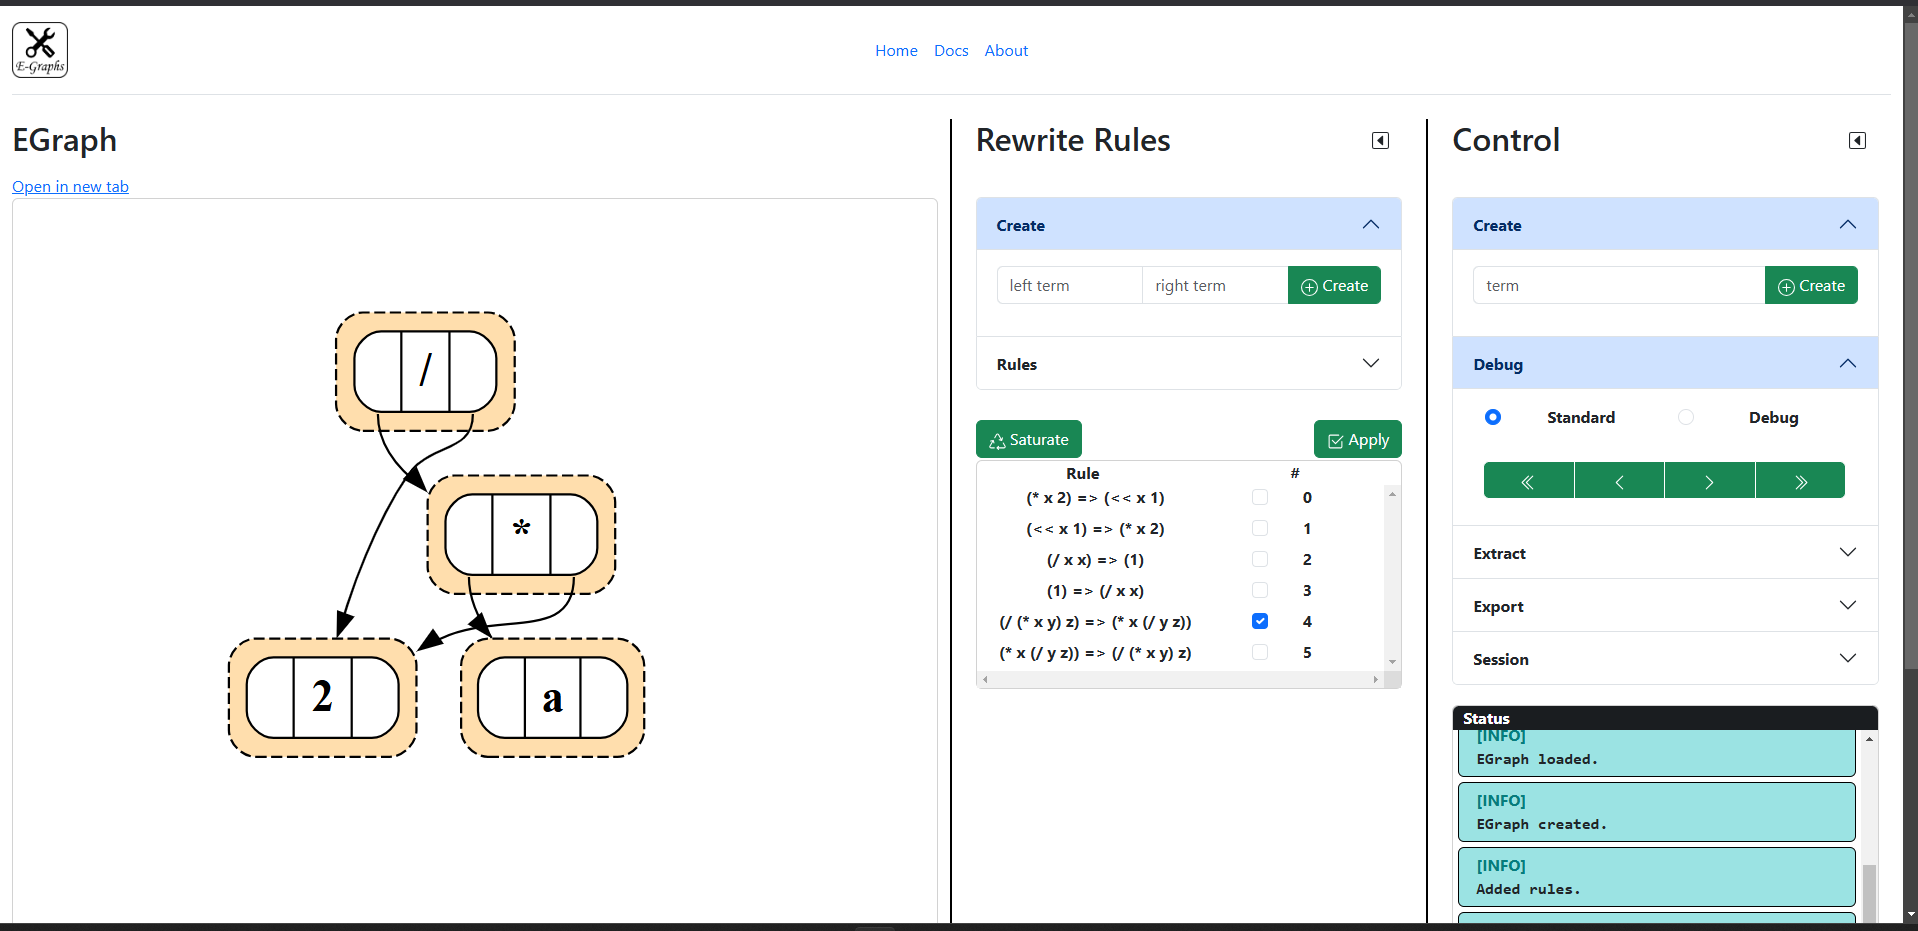
\includegraphics[scale=0.45]{../fig/website.png}
% \caption{Website beim Start des Servers}
% \label{fig:website}
% % \end{figure}
% \end{sidewaysfigure}

\newpage
\begin{figure}[H]
\centering
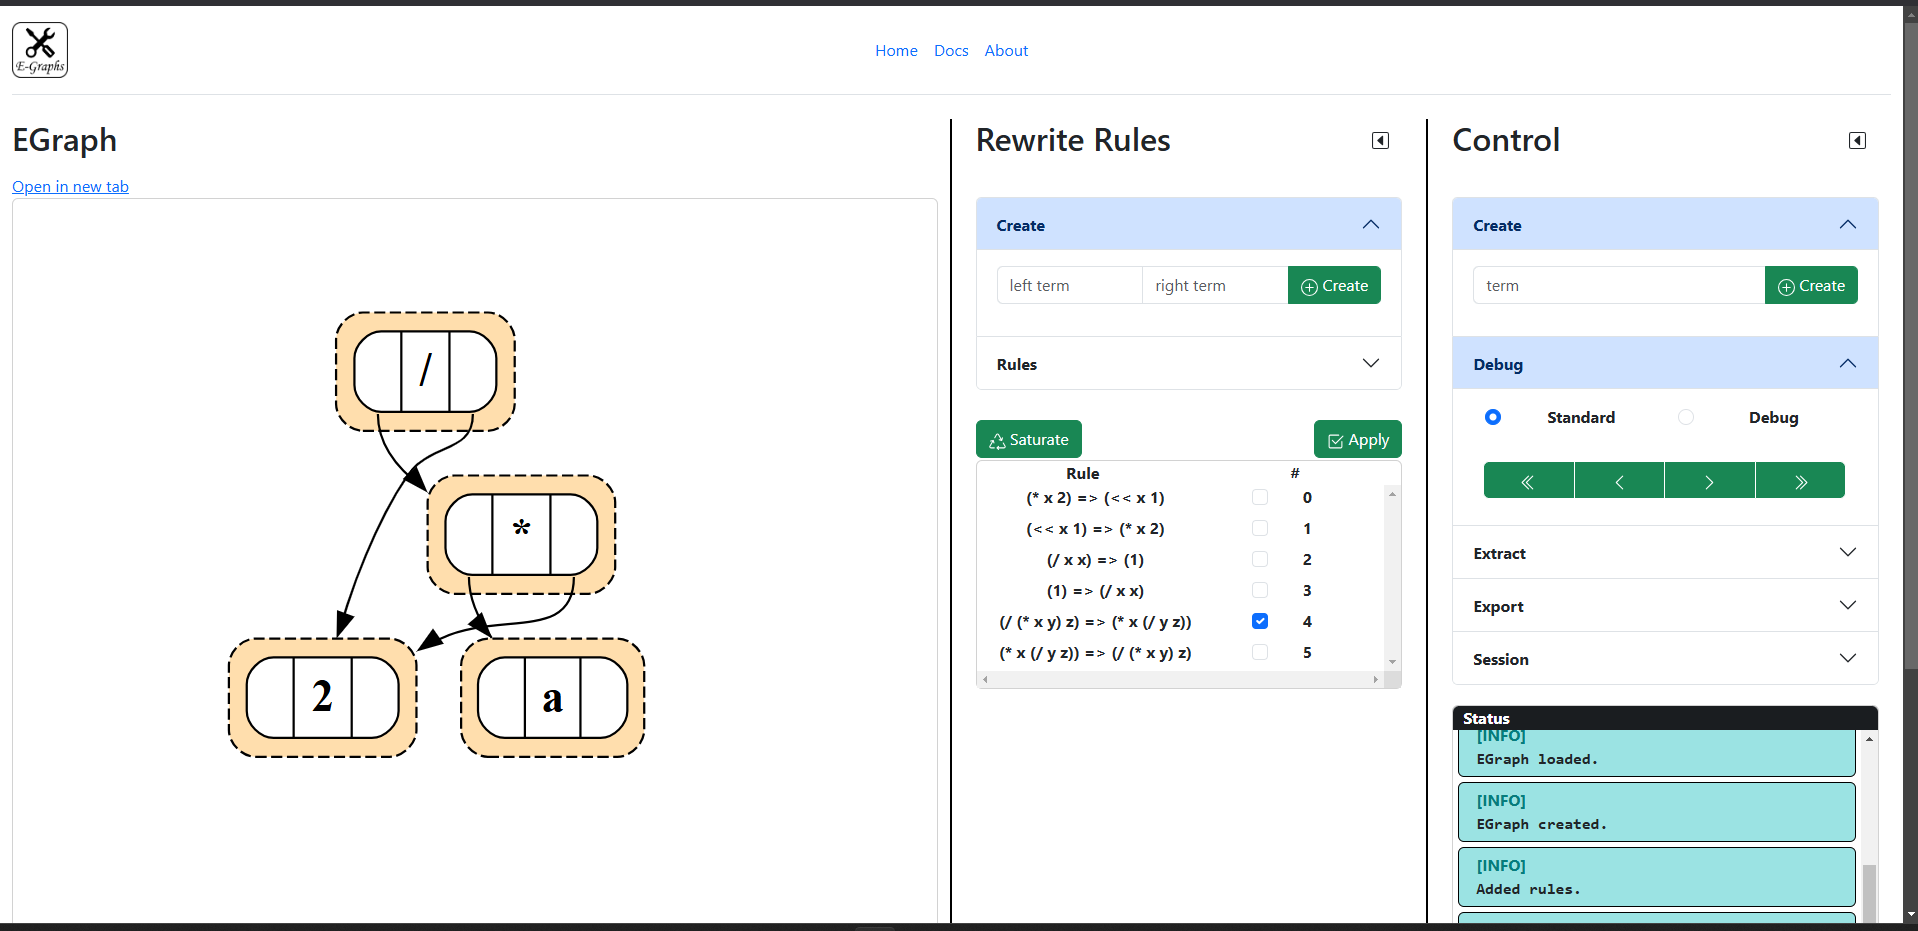
\includegraphics[scale=0.42, angle=90]{../fig/website.png}
\caption{Website beim Start des Servers}
\label{fig:website}
\end{figure}
\newpage


\subsubsection{JavaScript}

\subsubsection{Dokumentation}





% Die Benutzeroberfläche besteht aus einer Website, die im Browser läuft. Näheres zu dieser Entscheidung kann in Kapitel \ref{sec:entscheidungenundprobleme} nachgelesen werden.



